% !TeX spellcheck = en_US
% !TeX encoding = UTF-8
% !TeX program = xelatex
% TODO Change language to en_GB (recommended) or en_US for English documents
\documentclass[11pt,a4paper,oneside]{report}             % Single-side
%\documentclass[11pt,a4paper,twoside,openright]{report}  % Duplex

% thanks to http://tex.stackexchange.com/a/47579/71109
\usepackage{tikz}
\usetikzlibrary{automata,positioning}
\usepackage{marvosym}
\usepackage{float}
\usepackage{ifxetex}
\usepackage{ifluatex}
\newtheorem{prop}{Proposition}
\usepackage[ruled,linesnumbered]{algorithm2e}
\newif\ifxetexorluatex % a new conditional starts as false
\ifnum 0\ifxetex 1\fi\ifluatex 1\fi>0
   \xetexorluatextrue
\fi

\ifxetexorluatex
  \usepackage{fontspec}
\else
  \usepackage[T1]{fontenc}
  \usepackage[utf8]{inputenc}
  \usepackage[lighttt]{lmodern}
\fi

\usepackage[english,magyar]{babel} % Alapértelmezés szerint utoljára definiált nyelv lesz aktív, de később külön beállítjuk az aktív nyelvet.

%\usepackage{cmap}
\usepackage{amsfonts,amsmath, wasysym, amssymb, stmaryrd} % Mathematical symbols.
%\usepackage[ruled,boxed,resetcount,linesnumbered]{algorithm2e} % For pseudocodes. % beware: this is not compatible with LuaLaTeX, see http://tex.stackexchange.com/questions/34814/lualatex-and-algorithm2e
\usepackage{booktabs} % For publication quality tables for LaTeX
\usepackage{graphicx}

%\usepackage{fancyhdr}
%\usepackage{lastpage}

\usepackage{anysize}
%\usepackage{sectsty}
\usepackage{setspace} % For setting line spacing

\usepackage[unicode]{hyperref} % For hyperlinks in the generated document.
\usepackage{xcolor}
\usepackage{listings} % For source code snippets.

\usepackage[amsmath,thmmarks]{ntheorem} % Theorem-like environments.

\usepackage[hang]{caption}

\singlespacing

\newcommand{\selecthungarian}{
	\selectlanguage{magyar}
	\setlength{\parindent}{2em}
	\setlength{\parskip}{0em}
	\frenchspacing
}

\newcommand{\selectenglish}{
	\selectlanguage{english}
	\setlength{\parindent}{0em}
	\setlength{\parskip}{0.5em}
	\nonfrenchspacing
	\renewcommand{\figureautorefname}{Figure}
	\renewcommand{\tableautorefname}{Table}
	\renewcommand{\partautorefname}{Part}
	\renewcommand{\chapterautorefname}{Chapter}
	\renewcommand{\sectionautorefname}{Section}
	\renewcommand{\subsectionautorefname}{Section}
	\renewcommand{\subsubsectionautorefname}{Section}
}

\usepackage[numbers]{natbib}
\usepackage{xspace}


%TODO Set the main variables
\newcommand{\vikszerzoVezeteknev}{Barcsa-Szabó}
\newcommand{\vikszerzoKeresztnev}{Áron}

\newcommand{\vikkonzulensAMegszolitas}{}
\newcommand{\vikkonzulensAVezeteknev}{Farkas}
\newcommand{\vikkonzulensAKeresztnev}{Rebeka}

\newcommand{\vikkonzulensBMegszolitas}{Dr.~}
\newcommand{\vikkonzulensBVezeteknev}{Vörös}
\newcommand{\vikkonzulensBKeresztnev}{András}

\newcommand{\vikkonzulensCMegszolitas}{}
\newcommand{\vikkonzulensCVezeteknev}{}
\newcommand{\vikkonzulensCKeresztnev}{}

\newcommand{\vikcim}{Supporting system design with automaton learning algorithms} % Cím
\newcommand{\viktanszek}{\bmemit} % Tanszék
\newcommand{\vikdoktipus}{\bsc} % Dokumentum típusa (\bsc vagy \msc)
\newcommand{\vikmunkatipusat}{szakdolgozatot} % a "hallgató nyilatkozat" részhez: szakdolgozatot vagy diplomatervet

%--------------------------------------------------------------------------------------
% TDK-specifikus változók
%--------------------------------------------------------------------------------------
\newcommand{\tdkszerzoB}{Második Szerző} % Második szerző neve; hagyd üresen, ha egyedül írtad a TDK-t.
\newcommand{\tdkev}{2014} % A dolgozat írásának éve (pl. "2014") (Ez OTDK-nál eltérhet az aktuális évtől.)

% További adatok az OTDK címlaphoz (BME-s TDK-hoz nem kell kitölteni)
\newcommand{\tdkevfolyamA}{IV} % Első szerző évfolyama, római számmal (pl. IV).
\newcommand{\tdkevfolyamB}{III} % Második szerző évfolyama, római számmal (pl. III).
\newcommand{\tdkkonzulensbeosztasA}{egyetemi tanár} % Első konzulens beosztása (pl. egyetemi docens)
\newcommand{\tdkkonzulensbeosztasB}{doktorandusz} % Második konzulens beosztása (pl. egyetemi docens)

\newcommand{\szerzoMeta}{\vikszerzoVezeteknev{} \vikszerzoKeresztnev} % egy szerző esetén
%\newcommand{\szerzoMeta}{\vikszerzoVezeteknev{} \vikszerzoKeresztnev, \tdkszerzoB} % két szerző esetén

%TODO Language configuration -- choose one
% Beállítások magyar nyelvű dolgozathoz
%%--------------------------------------------------------------------------------------
% Elnevezések
%--------------------------------------------------------------------------------------
\newcommand{\bme}{Budapesti Műszaki és Gazdaságtudományi Egyetem}
\newcommand{\vik}{Villamosmérnöki és Informatikai Kar}

\newcommand{\bmemit}{Méréstechnika és Információs Rendszerek Tanszék}

\newcommand{\keszitette}{Készítette}
\newcommand{\konzulens}{Konzulens}

\newcommand{\bsc}{Szakdolgozat}
\newcommand{\msc}{Diplomaterv}
\newcommand{\tdk}{TDK dolgozat}
\newcommand{\bsconlab}{BSc Önálló laboratórium}
\newcommand{\msconlabi}{MSc Önálló laboratórium 1.}
\newcommand{\msconlabii}{MSc Önálló laboratórium 2.}

\newcommand{\pelda}{Példa}
\newcommand{\definicio}{Definíció}
\newcommand{\tetel}{Tétel}

\newcommand{\bevezetes}{Bevezetés}
\newcommand{\koszonetnyilvanitas}{Köszönetnyilvánítás}
\newcommand{\fuggelek}{Függelék}

% Opcionálisan átnevezhető címek
%\addto\captionsmagyar{%
%\renewcommand{\listfigurename}{Saját ábrajegyzék cím}
%\renewcommand{\listtablename}{Saját táblázatjegyzék cím}
%\renewcommand{\bibname}{Saját irodalomjegyzék név}
%}

\newcommand{\szerzo}{\vikszerzoVezeteknev{} \vikszerzoKeresztnev}
\newcommand{\vikkonzulensA}{\vikkonzulensAMegszolitas\vikkonzulensAVezeteknev{} \vikkonzulensAKeresztnev}
\newcommand{\vikkonzulensB}{\vikkonzulensBMegszolitas\vikkonzulensBVezeteknev{} \vikkonzulensBKeresztnev}
\newcommand{\vikkonzulensC}{\vikkonzulensCMegszolitas\vikkonzulensCVezeteknev{} \vikkonzulensCKeresztnev}

\newcommand{\selectthesislanguage}{\selecthungarian}

\bibliographystyle{huplain}

\def\lstlistingname{lista}

\newcommand{\appendixnumber}{6}  % a fofejezet-szamlalo az angol ABC 6. betuje (F) lesz

% Settings for English documents
%--------------------------------------------------------------------------------------
% Elnevezések
%--------------------------------------------------------------------------------------
\newcommand{\bme}{Budapest University of Technology and Economics}
\newcommand{\vik}{Faculty of Electrical Engineering and Informatics}

\newcommand{\bmemit}{Department of Measurement and Information Systems}

\newcommand{\keszitette}{Author}
\newcommand{\konzulens}{Advisor}

\newcommand{\bsc}{Bachelor's Thesis}
\newcommand{\msc}{Master's Thesis}
\newcommand{\tdk}{Scientific Students' Association Report}
\newcommand{\bsconlab}{BSc Project Laboratory}
\newcommand{\msconlabi}{MSc Project Laboratory 1}
\newcommand{\msconlabii}{MSc Project Laboratory 2}

\newcommand{\pelda}{Example}
\newcommand{\definicio}{Definition}
\newcommand{\tetel}{Theorem}

\newcommand{\bevezetes}{Introduction}
\newcommand{\koszonetnyilvanitas}{Acknowledgements}
\newcommand{\fuggelek}{Appendix}

% Optional custom titles
%\addto\captionsenglish{%
%\renewcommand*{\listfigurename}{Your list of figures title}
%\renewcommand*{\listtablename}{Your list of tables title}
%\renewcommand*{\bibname}{Your bibliography title}
%}

\newcommand{\szerzo}{\vikszerzoKeresztnev{} \vikszerzoVezeteknev}
\newcommand{\vikkonzulensA}{\vikkonzulensAMegszolitas\vikkonzulensAKeresztnev{} \vikkonzulensAVezeteknev}
\newcommand{\vikkonzulensB}{\vikkonzulensBMegszolitas\vikkonzulensBKeresztnev{} \vikkonzulensBVezeteknev}
\newcommand{\vikkonzulensC}{\vikkonzulensCMegszolitas\vikkonzulensCKeresztnev{} \vikkonzulensCVezeteknev}

\newcommand{\selectthesislanguage}{\selectenglish}

\bibliographystyle{plainnat}

\newcommand{\ie}{i.e.\@\xspace}
\newcommand{\Ie}{I.e.\@\xspace}
\newcommand{\eg}{e.g.\@\xspace}
\newcommand{\Eg}{E.g.\@\xspace}
\newcommand{\etal}{et al.\@\xspace}
\newcommand{\etc}{etc.\@\xspace}
\newcommand{\vs}{vs.\@\xspace}
\newcommand{\viz}{viz.\@\xspace} % videlicet
\newcommand{\cf}{cf.\@\xspace} % confer
\newcommand{\Cf}{Cf.\@\xspace}
\newcommand{\wrt}{w.r.t.\@\xspace} % with respect to
\newcommand{\approximately}{approx.\@\xspace}

\newcommand{\appendixnumber}{1}  % a fofejezet-szamlalo az angol ABC 1. betuje (A) lesz


%--------------------------------------------------------------------------------------
% Page layout setup
%--------------------------------------------------------------------------------------
% we need to redefine the pagestyle plain
% another possibility is to use the body of this command without \fancypagestyle
% and use \pagestyle{fancy} but in that case the special pages
% (like the ToC, the References, and the Chapter pages)remain in plane style

\pagestyle{plain}
\marginsize{35mm}{25mm}{15mm}{15mm}

\setcounter{tocdepth}{3}
%\sectionfont{\large\upshape\bfseries}
\setcounter{secnumdepth}{3}

\sloppy % Margón túllógó sorok tiltása.
\widowpenalty=10000 \clubpenalty=10000 %A fattyú- és árvasorok elkerülése
\def\hyph{-\penalty0\hskip0pt\relax} % Kötőjeles szavak elválasztásának engedélyezése


%--------------------------------------------------------------------------------------
% Setup hyperref package
%--------------------------------------------------------------------------------------
\hypersetup{
    % bookmarks=true,            % show bookmarks bar?
    unicode=true,              % non-Latin characters in Acrobat's bookmarks
    pdftitle={\vikcim},        % title
    pdfauthor={\szerzoMeta},    % author
    pdfsubject={\vikdoktipus}, % subject of the document
    pdfcreator={\szerzoMeta},   % creator of the document
    pdfproducer={},    % producer of the document
    pdfkeywords={},    % list of keywords (separate then by comma)
    pdfnewwindow=true,         % links in new window
    colorlinks=true,           % false: boxed links; true: colored links
    linkcolor=black,           % color of internal links
    citecolor=black,           % color of links to bibliography
    filecolor=black,           % color of file links
    urlcolor=black             % color of external links
}


%--------------------------------------------------------------------------------------
% Set up listings
%--------------------------------------------------------------------------------------
\definecolor{lightgray}{rgb}{0.95,0.95,0.95}
\lstset{
	basicstyle=\scriptsize\ttfamily, % print whole listing small
	keywordstyle=\color{black}\bfseries, % bold black keywords
	identifierstyle=, % nothing happens
	% default behavior: comments in italic, to change use
	% commentstyle=\color{green}, % for e.g. green comments
	stringstyle=\scriptsize,
	showstringspaces=false, % no special string spaces
	aboveskip=3pt,
	belowskip=3pt,
	backgroundcolor=\color{lightgray},
	columns=flexible,
	keepspaces=true,
	escapeinside={(*@}{@*)},
	captionpos=b,
	breaklines=true,
	frame=single,
	float=!ht,
	tabsize=2,
	literate=*
		{á}{{\'a}}1	{é}{{\'e}}1	{í}{{\'i}}1	{ó}{{\'o}}1	{ö}{{\"o}}1	{ő}{{\H{o}}}1	{ú}{{\'u}}1	{ü}{{\"u}}1	{ű}{{\H{u}}}1
		{Á}{{\'A}}1	{É}{{\'E}}1	{Í}{{\'I}}1	{Ó}{{\'O}}1	{Ö}{{\"O}}1	{Ő}{{\H{O}}}1	{Ú}{{\'U}}1	{Ü}{{\"U}}1	{Ű}{{\H{U}}}1
}


%--------------------------------------------------------------------------------------
% Set up theorem-like environments
%--------------------------------------------------------------------------------------
% Using ntheorem package -- see http://www.math.washington.edu/tex-archive/macros/latex/contrib/ntheorem/ntheorem.pdf

\theoremstyle{plain}
\theoremseparator{.}
\newtheorem{example}{\pelda}

\theoremseparator{.}
%\theoremprework{\bigskip\hrule\medskip}
%\theorempostwork{\hrule\bigskip}
\theorembodyfont{\upshape}
\theoremsymbol{{\large \ensuremath{\centerdot}}}
\newtheorem{definition}{\definicio}

\theoremseparator{.}
%\theoremprework{\bigskip\hrule\medskip}
%\theorempostwork{\hrule\bigskip}
\newtheorem{theorem}{\tetel}


%--------------------------------------------------------------------------------------
% Some new commands and declarations
%--------------------------------------------------------------------------------------
\newcommand{\code}[1]{{\upshape\ttfamily\scriptsize\indent #1}}
\newcommand{\doi}[1]{DOI: \href{http://dx.doi.org/\detokenize{#1}}{\raggedright{\texttt{\detokenize{#1}}}}} % A hivatkozások közt így könnyebb DOI-t megadni.

\DeclareMathOperator*{\argmax}{arg\,max}
%\DeclareMathOperator*[1]{\floor}{arg\,max}
\DeclareMathOperator{\sign}{sgn}
\DeclareMathOperator{\rot}{rot}


%--------------------------------------------------------------------------------------
% Setup captions
%--------------------------------------------------------------------------------------
\captionsetup[figure]{
	width=.75\textwidth,
	aboveskip=10pt}

\renewcommand{\captionlabelfont}{\bf}
%\renewcommand{\captionfont}{\footnotesize\it}

%--------------------------------------------------------------------------------------
% Hyphenation exceptions
%--------------------------------------------------------------------------------------
\hyphenation{Shakes-peare Mar-seilles ár-víz-tű-rő tü-kör-fú-ró-gép}


\author{\vikszerzo}
\title{\viktitle}

%--------------------------------------------------------------------------------------
% Table of contents and the main text
%--------------------------------------------------------------------------------------
\begin{document}

\pagenumbering{gobble}

%TODO These includes define guidelines -- remove these
%~~~~~~~~~~~~~~~~~~~~~~~~~~~~~~~~~~~~~~~~~~~~~~~~~~~~~~~~~~~~~~~~~~~~~~~~~~~~~~~~~~~~~~

\selectthesislanguage

%TODO Titlepage -- choose one from below
%~~~~~~~~~~~~~~~~~~~~~~~~~~~~~~~~~~~~~~~~~~~~~~~~~~~~~~~~~~~~~~~~~~~~~~~~~~~~~~~~~~~~~~
\hypersetup{pageanchor=false}
%--------------------------------------------------------------------------------------
%	The title page
%--------------------------------------------------------------------------------------
\begin{titlepage}
\begin{center}

\includegraphics[width=60mm,keepaspectratio]{figures/bme_logo.pdf}\\
\vspace{0.3cm}
\textbf{\bme}\\
\textmd{\vik}\\
\textmd{\viktanszek}\\[5cm]

\vspace{0.4cm}
{\huge \bfseries \vikcim}\\[0.8cm]
\vspace{0.5cm}
\textsc{\Large \vikdoktipus}\\[4cm]

{
	\renewcommand{\arraystretch}{0.85}
	\begin{tabular}{cc}
	 \makebox[7cm]{\emph{\keszitette}} & \makebox[7cm]{\emph{\konzulens}} \\ \noalign{\smallskip}
	 \makebox[7cm]{\szerzo} & \makebox[7cm]{\vikkonzulensA} \\
	  & \makebox[7cm]{\vikkonzulensB} \\
	  & \makebox[7cm]{\vikkonzulensC} \\
	\end{tabular}
}

\vfill
{\large \today}
\end{center}
\end{titlepage}
\hypersetup{pageanchor=false}

		   % Szakdolgozat/Diplomaterv címlap
%%% TDK címlap
\begin{titlepage}
  \begin{center}  
  
\includegraphics[width=7cm]{./figures/bme_logo.pdf}
  \vspace{0.3cm}
  
  \bme \\
  \vik \\
  \viktanszek \\
  \vspace{5cm}
  
  \huge {\vikcim}
  \vspace{1.5cm}
  
  \large {\textbf{\tdk}}
  \vfill
    
  {\Large 
  	\keszitette: \\ \vspace{0.3cm}
  	\szerzo \\
	\tdkszerzoB \\
  	\vspace{1.5cm}
  	\konzulens: \\ \vspace{0.3cm}
  	\vikkonzulensA \\
  	\vikkonzulensB \\
  }
  
  \vspace{2cm}
  \large {\tdkev}
 \end{center}
\end{titlepage}
%% Címlap vége
	% TDK címlap
%%% OTDK külső címlap
\begin{titlepage}
  	$\;$ 
	\vspace{5cm}
	
	\begin{center}
	\Huge
	\textbf{TDK-dolgozat}\let\thefootnote\relax\footnote{A dolgozat bemutatását a XXXXXXXXX  ``Lorem ipsum dolor sit amet'' című program támogatta.}
	\end{center}
	
	\vspace{13cm}
	
	\Large
	\hspace{8cm} \szerzo
	
	\hspace{8cm} \tdkszerzoB
	
	\hspace{8cm} \tdkev.
\end{titlepage}

\newpage
\thispagestyle{empty}


%% OTDK belső címlap
\begin{titlepage}
  \begin{center}  
  
\includegraphics[width=7cm]{./figures/bme_logo.pdf}
  \vspace{0.3cm}
  
  \bme \\
  \vik \\
  \viktanszek \\
  \vspace{3.5cm}
  
  \huge {\vikcim}
  \vspace{1.5cm}
  
  \large {\textbf{\vikdoktipus}}
  \vfill
    
  {\Large 
  	{\large \keszitette:} \\ \vspace{0.2cm}
  	\szerzo \\ \tdkevfolyamA. évfolyam \\
	\vspace{0.5cm}
	\tdkszerzoB \\ \tdkevfolyamB. évfolyam \\
  	\vspace{1.5cm}
  	{\large \konzulens:} \\ \vspace{0.2cm}
  	\vikkonzulensA,\\ \tdkkonzulensbeosztasA \\
  	\vspace{0.5cm}
  	\vikkonzulensB,\\ \tdkkonzulensbeosztasB \\
  }
  
  \vspace{2cm}
  \large {\tdkev.}
  
 \end{center}
\end{titlepage}   % OTDK címlap


% Table of Contents
%~~~~~~~~~~~~~~~~~~~~~~~~~~~~~~~~~~~~~~~~~~~~~~~~~~~~~~~~~~~~~~~~~~~~~~~~~~~~~~~~~~~~~~
\tableofcontents\vfill


% Declaration and Abstract
%~~~~~~~~~~~~~~~~~~~~~~~~~~~~~~~~~~~~~~~~~~~~~~~~~~~~~~~~~~~~~~~~~~~~~~~~~~~~~~~~~~~~~~
\selectlanguage{magyar}
\pagenumbering{gobble}
%--------------------------------------------------------------------------------------
% Nyilatkozat
%--------------------------------------------------------------------------------------
\begin{center}
\large
\textbf{HALLGATÓI NYILATKOZAT}\\
\end{center}

Alulírott \emph{\vikszerzoVezeteknev{} \vikszerzoKeresztnev}, szigorló hallgató kijelentem, hogy ezt a \vikmunkatipusat{} meg nem engedett segítség nélkül, saját magam készítettem, csak a megadott forrásokat (szakirodalom, eszközök stb.) használtam fel. Minden olyan részt, melyet szó szerint, vagy azonos értelemben, de átfogalmazva más forrásból átvettem, egyértelműen, a forrás megadásával megjelöltem.

Hozzájárulok, hogy a jelen munkám alapadatait (szerző(k), cím, angol és magyar nyelvű tartalmi kivonat, készítés éve, konzulens(ek) neve) a BME VIK nyilvánosan hozzáférhető elektronikus formában, a munka teljes szövegét pedig az egyetem belső hálózatán keresztül (vagy autentikált felhasználók számára) közzétegye. Kijelentem, hogy a benyújtott munka és annak elektronikus verziója megegyezik. Dékáni engedéllyel titkosított diplomatervek esetén a dolgozat szövege csak 3 év eltelte után válik hozzáférhetővé.

\begin{flushleft}
\vspace*{1cm}
Budapest, \today
\end{flushleft}

\begin{flushright}
 \vspace*{1cm}
 \makebox[7cm]{\rule{6cm}{.4pt}}\\
 \makebox[7cm]{\emph{\vikszerzoVezeteknev{} \vikszerzoKeresztnev}}\\
 \makebox[7cm]{hallgató}
\end{flushright}
\thispagestyle{empty}

\vfill
\clearpage
\thispagestyle{empty} % an empty page

\selectthesislanguage
 %TODO Hallgatói nyilatkozat -- TDK és OTDK esetén törlendő!
\pagenumbering{roman}
\setcounter{page}{1}

\selecthungarian

%----------------------------------------------------------------------------
% Abstract in Hungarian
%----------------------------------------------------------------------------
\chapter*{Kivonat}\addcontentsline{toc}{chapter}{Kivonat}

Informatikai rendszerek tervezése, fejlesztése modell-alapú technológiák segítségével hatékonyabbá tehető. A tervezett rendszerről rendelkezésre álló formális modell lehetővé teszi olyan feladatok automatizált végrehajtását, mint a helyességellenőrzés, kódgenerálás, valamint a rendszer kvalitatív és kvantitatív analízise.
\\\\
A rendszermodell reaktív komponensei (pl. kommunikációs protokollok) tipikusan állapot-alapú formalizmusokkal modellezhetők. Sokszor azonban a szükséges rendszermodell elkészítése nehéz feladat, hiszen ezen protokollokat kényelmesebb példalefutások alapján megtervezni. Tudomásom szerint az irodalomban még nincs olyan eszköz, mely lehetővé tenné egy rendszer(komponens) megtervezését példalefutások alapján.
\\\\
Munkám célja a rendszertervezés megkönnyítése, egy olyan szoftver létrehozásával, mely lehetővé teszi egy rendszer példalefutások alapján való megtervezését. A tervezett rendszer magját automatatanuló algoritmusok képzik, melyek erőssége éppen az, hogy állapot-alapú modelleket hoznak létre tervezett viselkedések alapján.
\\\\
A fenti cél megvalósítására a dolgozatomban bemutatok egy moduláris, kiterjeszthető és más szoftverekkel integrálható keretrendszert. Munkám során két algoritmust is implementáltam, melyek tetszőleges formalizmusokat képesek kezelni. Az elkészült keretrendszer hatékonyságát és alkalmazhatóságát mind elméleti szempontból, mind mérésekkel is igazoltam. 
\\
A bemutatott keretrendszer a rendszertervezés elősegítésén kívül az automatatanuló algoritmusok fejlesztését, összehasonlítását és tetszőleges célú felhasználását is lehetővé teszi.

%TODO: "olyan nincs, ami kiterjeszthető stb stb"
\vfill
\selectenglish


%----------------------------------------------------------------------------
% Abstract in English
%----------------------------------------------------------------------------
\chapter*{Abstract}\addcontentsline{toc}{chapter}{Abstract}

The design and development of technological systems can be made more efficient using model-based technologies. A formal model of the system under design makes the automation of tasks such as verification, code generation and qualitative, quantitative system-analysis possible.
\\\\
Reactive components of a system model (e.g. communication protocols) are typically modeled using state-based formalisms. However, the construction of such a system-model is often difficult, since these protocols are more straightforward to design using example runs of them. To the best of my knowledge, there is no tool in the literature capable of modeling system (components) using example runs.
\\\\
The objective of my work is to ease the process of system design by creating a software, which makes the modeling of a system using its example runs possible. The core of this framework is provided by automaton learning algorithms, the strength of which is exactly the creation of state-based models using behavioral information.
\\\\
To attain the above goal, I present a modular, extensible and easily integrable framework in this thesis. During my contribution, I've implemented two algorithms capable of handling arbitrary formalisms. I have confirmed the efficiency and applicability of these algorithms both theoretically, and by measurements.
\\
The presented framework, while capable of supporting system design, also enables the development, comparison and application of automaton learning algorithms.



\vfill
\selectthesislanguage

\newcounter{romanPage}
\setcounter{romanPage}{\value{page}}
\stepcounter{romanPage}    %TODO Összefoglaló -- TDK és OTDK esetén nem kötelező


% The main part of the thesis
%~~~~~~~~~~~~~~~~~~~~~~~~~~~~~~~~~~~~~~~~~~~~~~~~~~~~~~~~~~~~~~~~~~~~~~~~~~~~~~~~~~~~~~
\pagenumbering{arabic}

%TODO import your own content
%----------------------------------------------------------------------------
\chapter{Introduction}
%----------------------------------------------------------------------------

\section{Overview}



\section{Problémafelvetés}



\section{Célkitűzés}



\section{Contribution}



\section{Outline}

Chapter 2 provides an outline of the necessary technical background.

%----------------------------------------------------------------------------
\chapter{Background}
%----------------------------------------------------------------------------

This chapter provides some theoretical background of the contributions presented in this thesis. First of all, the necessary basics of formal language and automaton theory are introduced, afterwards we discuss automaton learning algorithms.

\section{Basics of automaton theory}

First, we introduce the fundamentals of formal language theory, which are essential in order to understand automaton theory. Atomic elements of formal languages are alphabets, characters and words.

\begin{definition}[Alphabet]
	Let $\Sigma$ be a finite, non-empty set. $\Sigma$ is an Alphabet, its elements are symbols or characters.
\end{definition}

\begin{definition}[Word]
	If $\Sigma$ is an alphabet, then any finite sequence comprised of the symbols of $\Sigma$ are words (or Strings). $\Sigma^{n}$ represents the set of every n length word in $\Sigma$. The set of every word under an alphabet, formally $\bigcup\limits_{n>0}^{} \Sigma^{n}$ is denoted by $\Sigma^{*}$.
\end{definition}

\begin{definition}[Formal Language]
	An arbitrary set of words under an Alphabet $\Sigma$ is a Language. Formally: $L\subseteq\Sigma^{*}$.
\end{definition}

We will expand on formal languages more once we have a basic understanding of automatons. 

Informally, Automatons, or automata are mathematical constructs which are able to determine if a sequence of inputs should be accepted or rejected. A bit more precisely, automata consist of states and is always in one of them. Starting from an initial state, based on the inputs received, the automaton changes, "moves" between states. Essentially, for every one of the inputs, based on the current state the automaton is in, it determines whether to keep, or change its current state. In order to determine if an input sequence should be accepted or not, some states are special, accepting states. If after processing a sequence of inputs, the final state of the automaton is accepting, the input sequence is accepted. If not, the input is rejected.


One of the most simple automaton is the Deterministic Finite Automaton.

\begin{definition}[Deterministic Finite Automaton]
	A Deterministic Finite Automaton is a Tuple of $ DFA=(S,s_{0},\Sigma,\delta,F) $, where: 
	\begin{itemize}
		\item S is a finite, non-epty set containing the states of the automaton,
		\item $s_{0} \in S$ is the initial state,
		\item $\Sigma$ is a finite Alphabet,
		\item $\delta: S\times \Sigma \to S$ is a transition function,
		\item $F\subseteq S$ is a set of the accepting states of the automaton. 
	\end{itemize}
\end{definition}


An example of a DFA (Deterministic Finite Automaton) from\cite{Steffen2011} can be seen in Example \ref{ex:dfaexample}.

\begin{example}
	\label{ex:dfaexample}
	See Fig. \ref{fig:dfaexample}. This example has four states, $S = \{q_0, q_1, q_2, q_3\}$ (hence $|S| = 4$). The initial state is marked by the start arrow, so $s_0 = q_0$. The alphabet can be inferred as $\Sigma = \{a, b\}$ because of the deterministic in Deterministic Finite Automaton, meaning every state must deterministically know what input causes what action. This means, that every state must have every member of the alphabet listed in its transitions. Transitions are visualized as $q_0$ $\xrightarrow[]{\text{a}}$ $q_1$ given by the transition function (in this example) $\delta(q_0, a) = q_1$. The whole of the transition function in a table form can be seen in Table \ref{tab:dfaexampledelta}. Finally, the accepting states, or in this case, accepting state of the automaton is $F = \{q_3\}$.
\end{example}
 

When talking about automata, it is important to discuss runs. A run of an automaton is to test for a certain input (word), if it is accepted or rejected. See Example \ref{ex:dfaruns}.

\begin{example}
	\label{ex:dfaruns}
	A run of Fig. \ref{fig:dfaexample} with an input of $\{a, a, a\}$ would (following the transition function) end in state $q_3$ meaning the input is accepted. A rejected input could be $\{a, b, b\}$, which would stop at state $q_1$, a non-accepting state. On deeper examination, one can see, that this automaton only accepts runs with inputs containing $4i+3 a$.
\end{example}

\begin{figure}[H]
	\centering
	\begin{tikzpicture}[shorten >=1pt,node distance=3cm,on grid,auto] 
	\node[state,initial] (q_0)   {$q_0$}; 
	\node[state] (q_1) [right=of q_0] {$q_1$}; 
	\node[state] (q_2) [below=of q_0] {$q_2$}; 
	\node[state,accepting](q_3) [right=of q_2] {$q_3$};
	\path[->] 
	(q_0) edge  node {a} (q_1)
	edge [loop below] node {b} ()
	(q_1) edge  node  {a} (q_2)
	edge [loop below] node {b} ()
	(q_2) edge  node [swap] {a} (q_3) 
	edge [loop above] node {b} ()
	(q_3) edge  node [swap] {a} (q_0)
	 edge [loop above] node {b} () ;
	\end{tikzpicture}
	\caption{A simple DFA}
	\label{fig:dfaexample}
\end{figure}

\begin{table}[H]
\centering
\begin{tabular}{|c|cccc|}
	\hline
	$\delta$ & $q_0$ & $q_1$ & $q_2$ & $q_3$\\ \cline{1-5}
	a & $q_1$ & $q_2$ & $q_3$ & $q_0$ \\	
	b & $q_0$ & $q_1$ & $q_2$ & $q_3$ \\	\hline
\end{tabular}
\caption{The transition function of the automaton seen in Fig. \ref{fig:dfaexample}}
\label{tab:dfaexampledelta}
\end{table}

DFAs are great to model system behavior based on inputs, but in order to work with reactive systems, we also need to handle outputs. Mealy machines are automata designed to do just this, while becoming more complicated with regard to accepting inputs.


\begin{definition}[Mealy machine]
	A Mealy machine or Mealy automaton is a Tuple of $ M=(S,s_{0},\Sigma,\Omega,\delta,\lambda) $, where:
	\begin{itemize}
		\item S is a finite, non-empty set containing the states of the automaton,
		\item $s_{0} \in S$ is the initial state,
		\item $\Sigma$ is the input alphabet of the automaton,
		\item $\Omega$ is the output alphabet of the automaton,
		\item $\delta: Q\times \Sigma \to Q$ is the transition function and
		\item $\lambda: Q\times \Sigma \to \Omega$ is the output function. 
	\end{itemize}
\end{definition}

Mealy machines can be regarded as deterministic finite automata over the union of the input alphabet and an output alphabet with just one rejection state, which is a sink, or more elegantly, with a partially defined transition relation. 

An example of a deterministic Mealy machine can be seen in Example \ref{ex:coffeemealy}.

\begin{example}
	\label{ex:coffeemealy}
	An example of a deterministic Mealy machine can be seen in Fig. \ref{fig:coffeemealy}. The formal definition of the automaton can be seen below.
	\begin{itemize} 
		\item $S = \{a, b, c, d, d', e, f\}$ 
		\item $s_0 = a$
		\item $\Sigma = \{water, pod, button, clean\}$
		\item $\Omega$ = \{$\checkmark$, \Coffeecup, $\star$\}
	\end{itemize}
	The transitions, as seen in Fig. \ref{fig:coffeemealy} are visualized as $s_0$ $\xrightarrow[]{\text{input/output}}$ $s_1$, which denotes the machine moving from state $s_0$ to state $s_1$ on the specified input, while causing the specified output. Also, some simplifications are done, e.g. in this transition: d $\xrightarrow[]{\text{\{water,pod\}/\checkmark}}$ d we see a visual simplification of having both transitions merged to one arrow, this is only for visual convenience. Fig. \ref{fig:coffeemealy} is also a great example of sinks, as seen in state f, the machine accepts anything, and never changes. This is a variation of the accepting state seen in DFAs.
\end{example}

\begin{figure}[H]
	\centering
	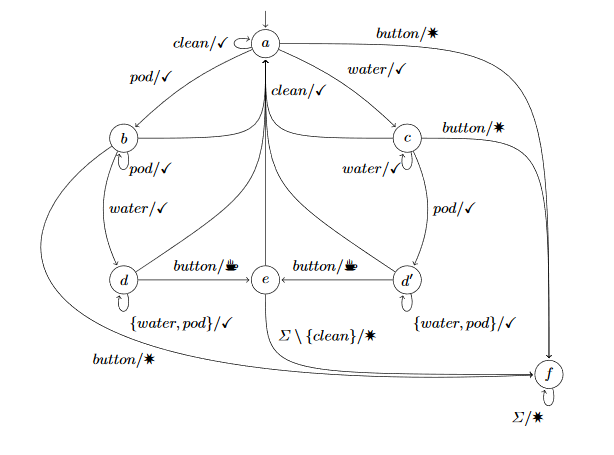
\includegraphics[width=0.7\linewidth]{content/coffeemealy}
	\caption{Mealy machine representing the functionality of a coffee machine.\cite{Steffen2011}}
	\label{fig:coffeemealy}
\end{figure}

Since automatons deal with alphabets, formal language theory is essential not only to work with them, but to build them efficiently. Often automata are used to model and test real-life systems. Naturally, questions of efficiency, correctness arise, which is why we will next expand on the relations of automatons and formal languages.

\begin{definition}[Recognized language of automata]
	The language $L\subseteq\Sigma$ containing all the accepted words by an automaton M is called the recognized language of the automaton. It is denoted by L(M) = L.
\end{definition}

\begin{definition}[Regular language]
	A formal language L is regular, iff there exists a Deterministic Finite Automaton M, for which L(M) = L, in other words, iff there exists a DFA with the recognized language of L.
\end{definition}

Next, we will introduce regularity to Mealy machines, which are a bit more complex in this regard.

In order to do this, we need to introduce some semantic helpers. $\delta^*$ is an extension of the $\delta$ transition function, as $\delta^*: S\times\Sigma^* \to S$ defined by $\delta^*(s,\epsilon) = s$ and $\delta^*(s, \alpha w) = \delta^*(\delta(s, \alpha), w)$, essentially giving us the state of the automaton after running an input sequence from a specified state. The same extension is done with the output function, as $\lambda^*: S\times\Sigma^* \to \Omega$, defined by $\lambda^*(s, \epsilon) = \varnothing$ and $\lambda^*(s, w\alpha) = \lambda(\delta^*(s, w), \alpha)$.



When monitoring the behavior of Mealy machines, one of the most important metrics given an input is not whether it is accepted or rejected (as it would be with a DFA), but rather what specific output was caused by an input. The behavior of a Mealy machine, a specific run of it, has a pattern of \textit{$i_1,o_1,i_2,o_2,..,i_n,o_n$}, where \textit{i} are inputs and \textit{o} are outputs. But in order to characterize these runs, we actually do not need every output from this pattern, we only need the final one. This means, that a $\llbracket M\rrbracket$: $\Sigma^*\to\Omega$ semantic functional fully captures the behavioral semantics of Mealy machines. We define $\llbracket M\rrbracket$: $\Sigma^*\to\Omega$ as  $\llbracket M\rrbracket$(w) = $\lambda^*(s_0, w)$. Informally,the  $\llbracket M\rrbracket$ functional accepts a set of inputs, and returns the last output given after running them from the initial state of the automaton.

\begin{example}
	Given the Mealy machine $M\textsubscript{coffeemachine}$ in Fig. \ref{fig:coffeemealy}, the runs:\\
	\null\qquad<clean, $\checkmark$>, \\
	\null\qquad<pod water button, \Coffeecup> \\
	are in $\llbracket M\textsubscript{coffeemachine}\rrbracket$, since these input words cause these outputs, while the runs\\
	\null\qquad<clean, \Coffeecup> and \\
	\null\qquad<water button button, $\checkmark$> \\
	are not, since these input sequences do not produce those outputs.
\end{example}

Now that we have the semantic functional $P:\Sigma^*\to\Omega$, we can introduce the concept of regularity to Mealy machines, but first, let's see what regularity means in DFAs.






\begin{definition}[Canonical automaton]
	An automaton accepting the language L is canonical iff it is minimal, and contains every other automaton that accepts L.
\end{definition}

\section{Automaton learning}



\paragraph{Automaton learning}  is the process of modeling a system without having specific knowledge of the internal workings of it. To accomplish this, we need to infer a model by observing its external behavior. This learned model is, as the name suggests, an automaton. 
\\Formally: Active  automata  learning is  concerned  with  the  problem  of  inferring  an automaton model for an unknown formal language $L$ over some alphabet $\Sigma$\cite{Howar2018}.
\\\\In order to monitor a system, we need a way of access to its behavioral information, for which there are two approaches, these separate the two types of automaton learning as well.

\paragraph{Passive automaton learning} is the case when the gathering of information is not part of the learning process, but rather a prerequisite to it. The learning is done on a pre-gathered positive an/or negative example set of the systems behavior. In passive automaton learning, the success of the process is not only determined by the efficiency of the algorithm, but the methodology and time used to gather the data.

\paragraph{Active automaton learning} is when the behavioral infromation is gathered by the learning algorithm in an "active" way via queries. For this there is a need to distinguish a learner and a teacher component, of which the second can answer basic questions about the system in real-time. 


\paragraph{MAT modell} Active automaton learning follows the MAT, or the Minimally Adequate Teacher model proposed by Dana Angluin\cite{ANGLUIN198787}. It separates the algorithm to a learner and a teacher, where the teacher can only answer the minimally adequate questions needed to learn the system. These two questions, or more precisely, queries are:


\paragraph{Membership query} Given a $w\in\Sigma^{*}$ word, it return the $o\in \Omega$ output corresponding to it, treating the word as a string of inputs.

\paragraph{Equivalence query} Given an $M$ hypothesis automaton, it tries to provide a counterexample $o\in\Omega$ and a $w\in\Sigma$ corresponding to it, where given the input $w$ to $M$ and the system, the output given by them differs. $o$ is the differring output given by the system. If no such counterexample can be found, M hypothesis is considered behaviorally identical to the monitored system.

\noindent The learner uses membership queries to build a hypothesis automaton, then refines these by equivalence queries. Once counterexamples can not be found this way, the learning terminates, the output is the current hypothesis.


\chapter{Contribution}

The main contribution in this thesis is to provide an active automaton learning framework, which can be used to support system design and analysis. This framework, since used in system design, is needed to be easily modifiable and extensible, while having the capability of handling any variation of formalisms systems might use.
\\\\
In order to tackle the problem of creating such a framework, I first needed to understand active automaton learning algorithms themselves.
\\
\section{Implementing a learning algorithm}

\begin{figure}
	\centering
	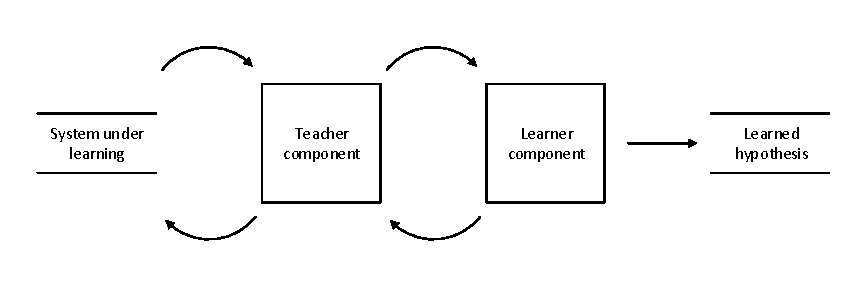
\includegraphics[width=1.0\linewidth]{figures/learningcomm}
	\caption{Data flow of active learning algorithms.}
	\label{fig:learningcomm}
\end{figure}

After processing the background knowledge seen in \cite{Steffen2011}, I decided to implement the most straightforward learning algorithm presented therein, the direct hypothesis construction algorithm.
\\
The first step was determining the formalisms used in this implementation, more specifically, the input and the output formalisms. Active automaton learning algorithms essentially have two endpoints: one being the input, reached through the teacher component, and the other being the output, where the learned hypothesis automaton is returned. This is illustrated in Fig. \ref{fig:learningcomm}. The teacher and learner component can handle abstraction, meaning the formalisms of the system under learning, or from now the input formalism, and the formalism of the learned hypothesis, or from now, the output formalism can both be arbitrary. Only implementing a specific algorithm, these formalisms needed to be specified. \\

Even if at first I was only implementing a single algorithm, the decisions on the formalism of this implementation was made with the future framework in mind. Since automaton learning algorithms can be  implemented on any type of automata, the easiest method would've been to implement DHC using deterministic finite automata. However, real-life reactive systems usually are better modeled using Mealy machines, hence the implementation was made using Mealy machines as both input and output formalisms.
\\
The first step of the implementation process was choosing the right tooling. This decision was also formed by the future system design perspective, which is why the Mealy machine implementation was done in Eclipse Modeling Framework.
\\\\
Eclipse Modeling Framework (EMF), or more specifically, EMF core, is an "abstraction for describing, composing, and manipulating structured information", essentially a tool for system modeling and code generation implemented in Java. Figure \ref*{fig:mealyecore} shows an UML class diagram of the metamodel I've created using the Ecore package of EMF core. 

\begin{figure}
	\centering
	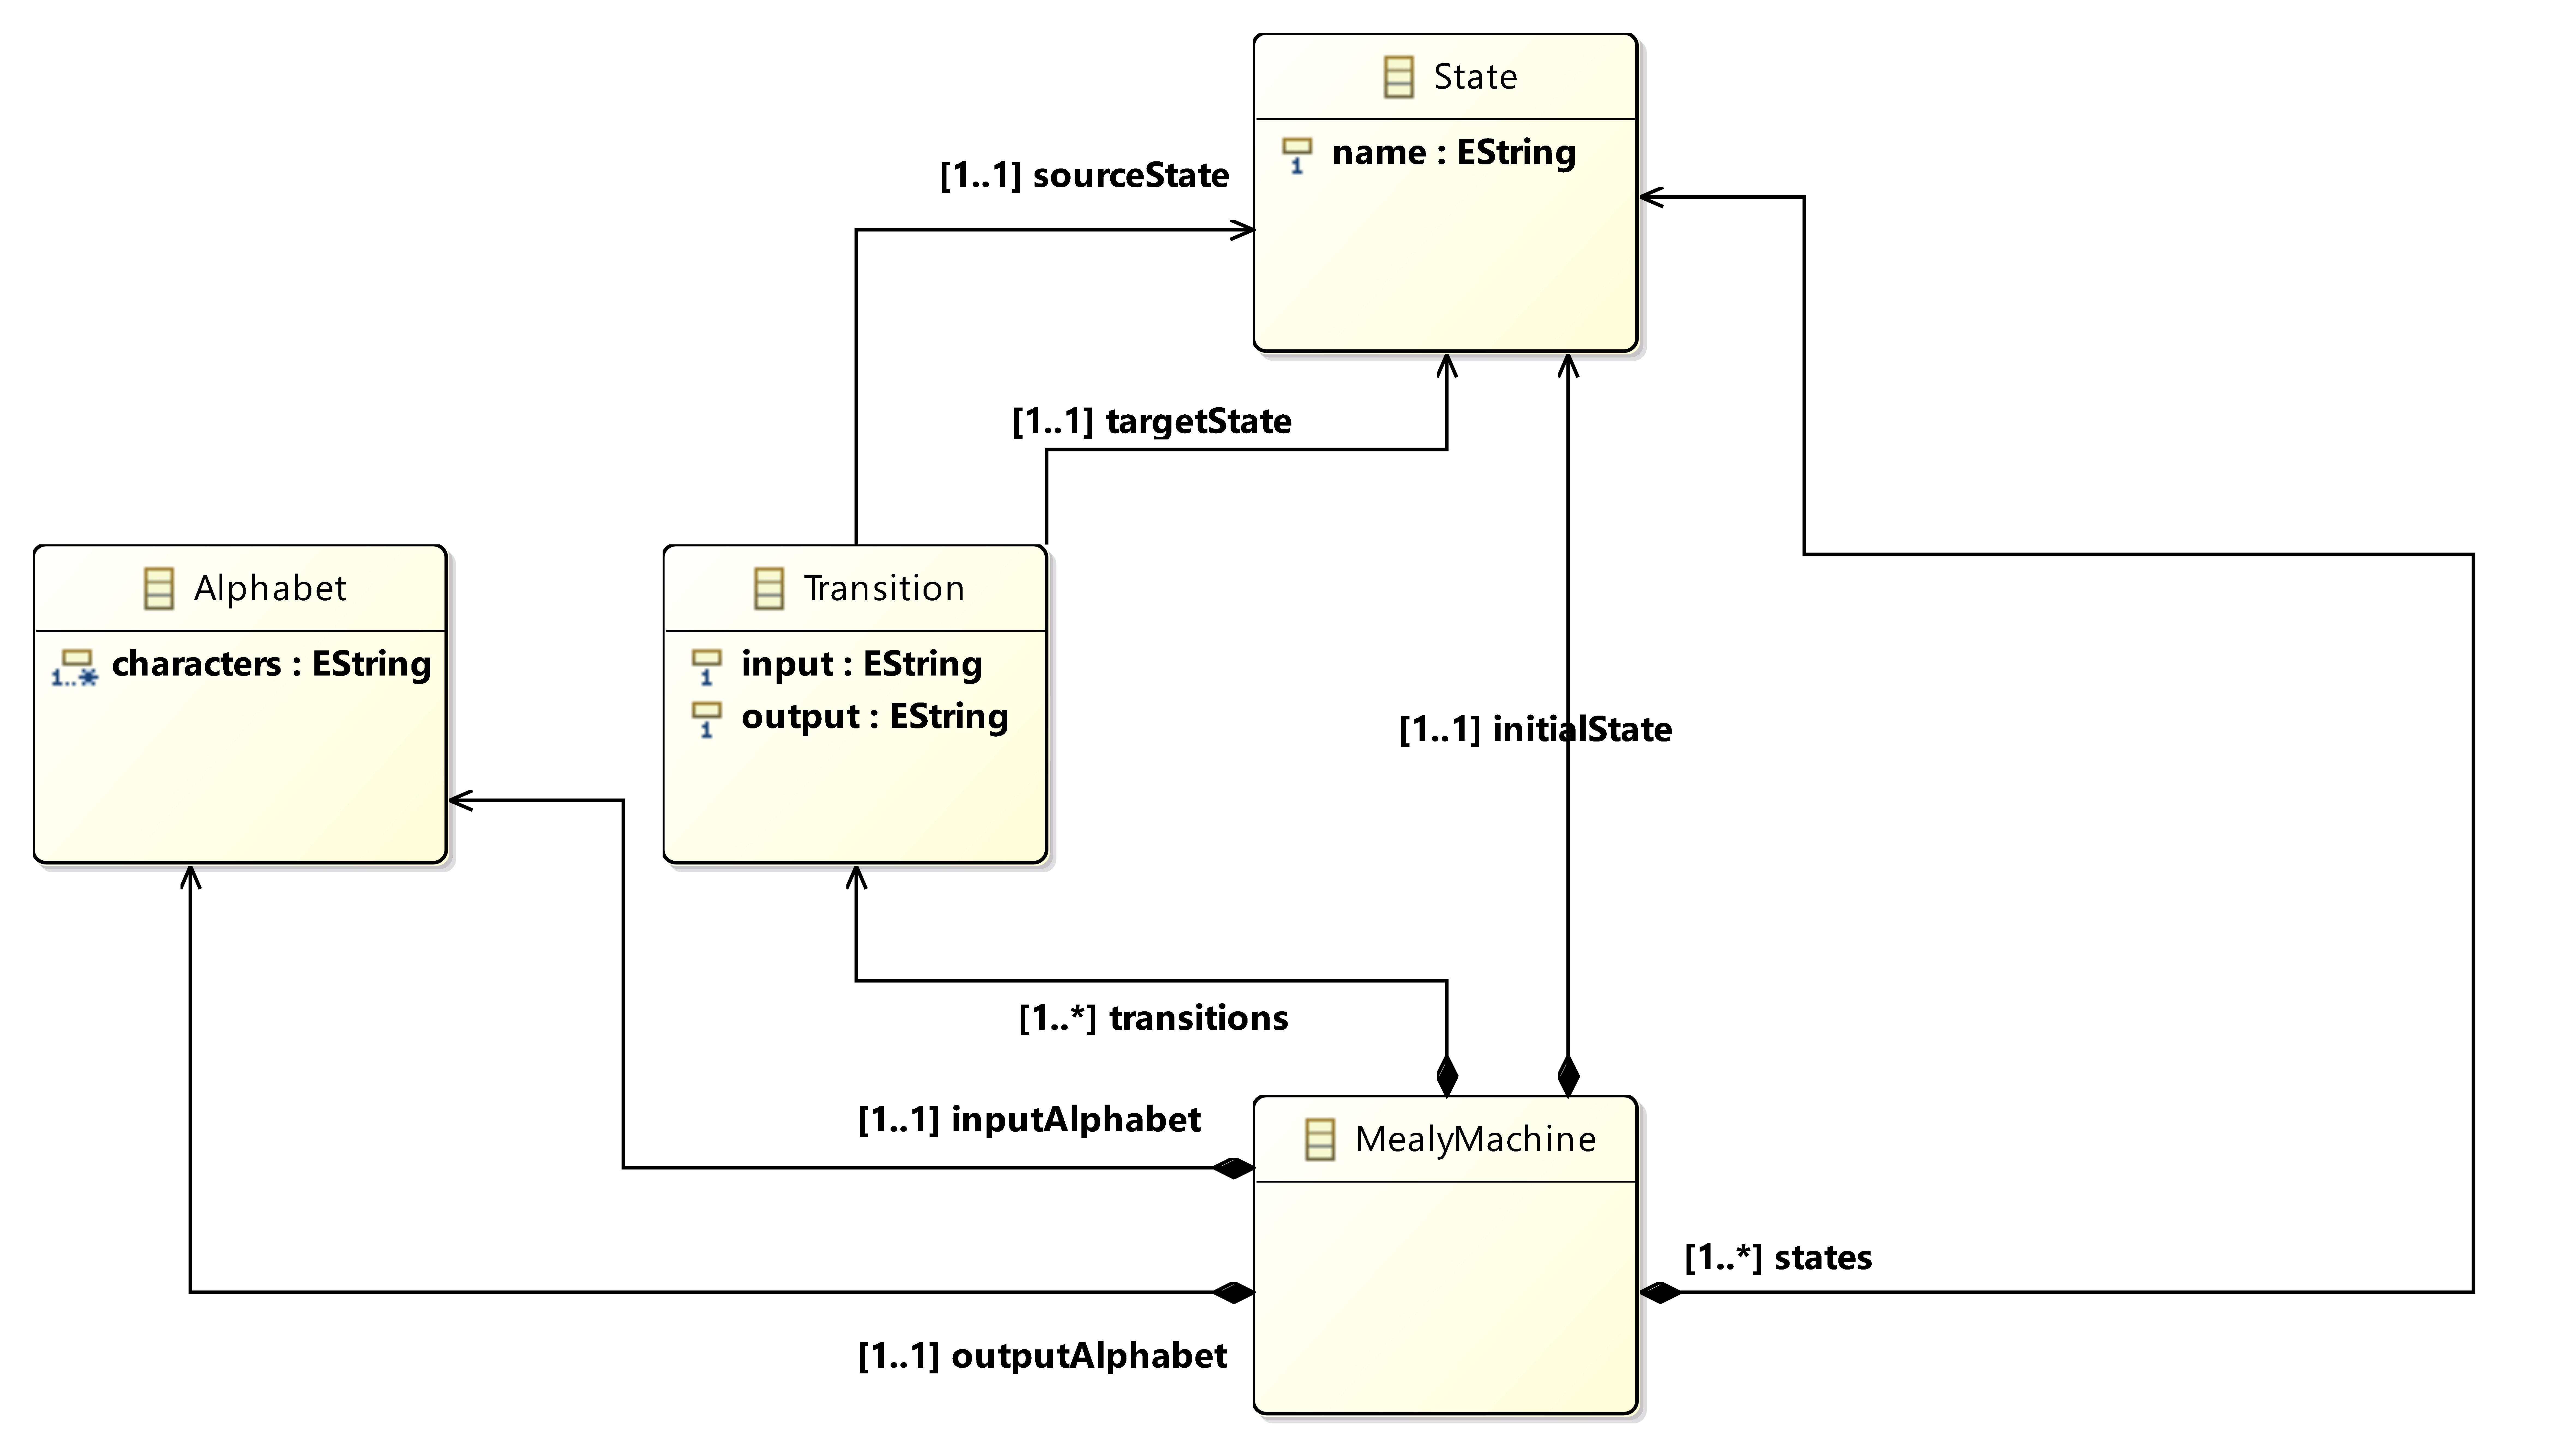
\includegraphics[width=1.0\linewidth]{figures/mealymodel}
	\caption{Ecore metamodel of Mealy machines.}
	\label{fig:mealyecore}
\end{figure}

In text, the Ecore model I've created uses Strings as distinguishers (on code generation, EString is converted to java.lang.String). States of the automaton, i.e. State objects are differentiated based on the name field. Note, that this is a transition-driven model of mealy machines, the Transition class stores the source and target states of the transition, as opposed to some models, where states store their own transition information (successors, predecessors) like nodes in a graph. This decision was based on the DHC algorithm, which while learning, stores traversal information itself, rather than asking for it, which is why ease of access is preferred as opposed to efficiency.
\\\\
Using EMF, I generated the class diagram seen in Fig. \ref{fig:mealyecore} into Java code. With this code, I implemented the direct hypothesis construction algorithm (in Java as well), without any framework whatsoever, only a single class accepting a MealyMachine object and constructing a Hypothesis MealyMachine object based off of it. In order to run and test this implementation, an example was needed, for which I chose the automaton seen in \ref{fig:coffeemealy}. Programmatically creating this example as an object is not a scalable solution, espetially regarding the future framework to be built, so I used Xtext, another tool, to solve this issue.
\\
Xtext is a framework for creating programming and domain-specific languages, which also has integration with EMF metamodels. Using this integration, I generated the Xtext grammar seen in Listing \ref{li:xtext}. In words, this  grammar describes a textual grammar in which instances of the metamodel seen in Fig. \ref{fig:mealyecore} can be stored. 



\begin{lstlisting}[caption=Xtext grammar describing Mealy machines.,label=li:xtext]
MealyMachine returns MealyMachine:
	'MealyMachine'
	'{'
		'initialState' initialState=State
		'states' '{' states+=State ( "," states+=State)* '}' 
		'inputAlphabet' inputAlphabet=Alphabet
		'outputAlphabet' outputAlphabet=Alphabet
		'transitions' '{' transitions+=Transition ( "," transitions+=Transition)* '}' 
	'}';
	
State returns State:
	{State}
	'State'
	name=EString;

Alphabet returns Alphabet:
	'Alphabet'
	'{'
		'characters' '{' characters+=EString ( "," characters+=EString)* '}' 
	'}';

Transition returns Transition:
	'Transition'
	'{'
		'input' input=EString
		'output' output=EString
		'sourceState' sourceState=[State|EString]
		'targetState' targetState=[State|EString]
	'}';

EString returns ecore::EString:
STRING | ID;
\end{lstlisting}

Utilizing the Xtext grammar in Listing \ref{li:xtext}, I created the input to be used by the implemented DHC, containing the formalized version of the automaton shown in Fig. \ref{fig:coffeemealy}. The input file can bee seen in Listing \ref{li:4ixtext}


\begin{lstlisting}[caption=The Mealy machine seen in Fig.\ref{fig:dfaexamplemealyver}.a in the form of the Xtext grammar described in Listing \ref{li:xtext}.,label=li:4ixtext]
	MealyMachine{
		initialState 
		State q0 states { State q0, State q1, State q2, State q3}
		inputAlphabet Alphabet { characters { a , b } }
		outputAlphabet Alphabet { characters { top , bot } }
		transitions{ 
		Transition { input a output top sourceState q0 targetState q1 } , 
		Transition { input b output top sourceState q0 targetState q0 } , 
		Transition { input a output top sourceState q1 targetState q2 } , 
		Transition { input b output top sourceState q1 targetState q1 } , 
		Transition { input a output bot sourceState q2 targetState q3 } , 
		Transition { input b output top sourceState q2 targetState q2 } , 
		Transition { input a output top sourceState q3 targetState q0 } , 
		Transition { input b output bot sourceState q3 targetState q3 } } }
\end{lstlisting}

Using the input file in Listing \ref{li:4ixtext} and converting it to a MealyMachine object using Xtext/EMF integration, the implemented DHC algorithm worked as intended. The execution of the algorithm returned with a new MealyMachine hypotesis object, which was the minimal version of the input automaton (seen in Fig. \ref{fig:coffeemealyminimal}). After the learning, the program wrote the learned hypothesis into a file in the same Xtext grammar the input was described in.\\ The overview of this implementation can be seen in Table \ref{tab:activelearningproto}.

\renewcommand{\tabularxcolumn}[1]{m{#1}}
\newcolumntype{Y}{>{\centering\arraybackslash}X}
\begin{table}[H]
	
	\begin{tabularx}{\columnwidth}{YYYYY}
		\hline
		\textbf{Algorithm} & \textbf{Input formalism} & \textbf{Output formalism} & \textbf{Input source} & \textbf{Output source}\\ \hline
		Direct Hypothesis Construction & Mealy machine & Mealy machine & Xtext & Xtext \\	\hline
	\end{tabularx}
	\caption{Overview of the prototype DHC algorithm implementation.}
	\label{tab:activelearningproto}
\end{table}

I used the experience gained during this prototype implementation to extend it into a framework.

\section{Automaton learning framework}
After implementing a singular active learning algorithm using fixed formalisms, I started designing an abstract framework to implement any algorithm using arbitrary formalisms. My desing decisions are mostly illustrated by Fig. \ref{fig:flowchartlearning}. The "Learner" and the "Teacher" components are both abstractions upon an algorithm, with two endpoints, one being the input, the other the output. Following this mindset, I first created a high-level model of the framework.

\subsection{High-level overview}

Since the implementation of the framework would be using Java as a language, the high-level view of it seen in Fig. \ref{fig:abstractoverview} is an UML class diagram of the packages and the relations between them, essentially being an overview of the modularization of the framework.

\begin{figure}
	\centering
	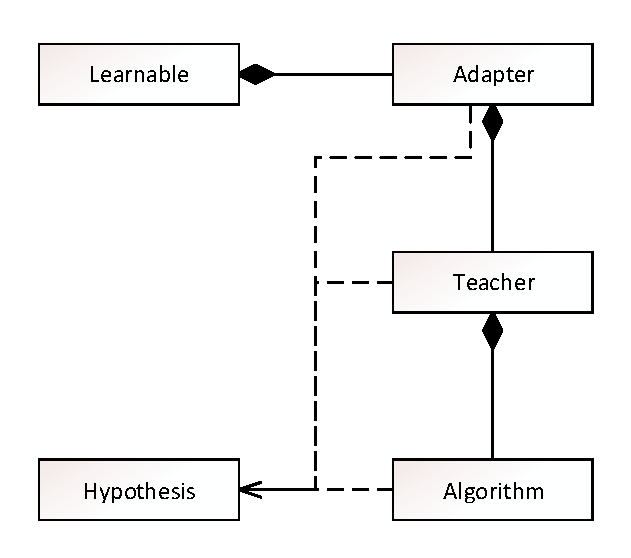
\includegraphics[width=0.5\linewidth]{figures/abstractoverview}
	\caption{Structure and relations of the packages comprising the framework.}
	\label{fig:abstractoverview}
\end{figure}

Note, that when comparing Fig. \ref{fig:abstractoverview} to Fig. \ref{fig:flowchartlearning}, the data flows identically. The Learnable package containing the input formalisms, and the Hypothesis package containing the output formalisms are used by the teacher (Teacher package) and the learner (Algorithm package). The package not represented on Fig. \ref{fig:flowchartlearning}, the Adapter package is used as an abstraction layer by which the algorithm and the teacher get separated from the input formalism. Since automaton learning algorithms have no direct access to the system under learning, they operate in a black-box way, this Adapter package is a useful addition, which unfortunately can not be used on the output layer. Hypothesis are directly accessed by the learning algorithms, they are constructed during the learning. While more specific abstractions were made (and can be seen later), no singular abstraction layer can be provided for every type of automaton and every type of learning algorithm the same way as for the input formalisms.
\\\\
The relations between the packages (modules) are straightforward. Composition is used, to indicate, that there is no Algorithm (learner) without a Teacher, there is no Teacher, without an Adapter, and there is no Adapter, without an input, a Learnable, to adapt. Algorithms of course depend on Hypothesis, and because of equivalence queries, which are later queried through the Teacher and Adapter components, they both also have a dependency on the Hypothesis package.

\subsection{Detailed overview of abstractions}


The diagram in Figure \ref{fig:abstractoverview} showed the modularization of the framework, which depend on the correct implementation of object-oriented architecture so the notated compositions and dependencies in Fig. \ref{fig:abstractoverview} are satisfied. These abstractions are defined and implemented in Java as abstract classes and interfaces seen in Fig. \ref{fig:abstractdetailedoverview}. The detailed descriptions of these abstractions are as follows.
\\
\begin{itemize}
	\item \textbf{Learnable:} The \emph{Learnable} interface is the input type used by the framework. It defines two generic parameters, \emph{I} is the character type of the regular language the Learnable represents, while \emph{O} is the character type by which actions are defined for the system under learning. The only method the interface defines is the \emph{getOutput()} method, which returns the output \emph{O} given by the system under learning for a specific sequence of inputs. Note, that while the word "output" is used, the \emph{O} it returns is the action the system takes for an input. If the system is represented as a DFA, this would be the state it moves to, if the system is represented as a Mealy machine, it would be an output.
	
	\item \textbf{Hypothesis:} The \emph{Hypothesis} abstract class is the output type used by the framework. The generic parameters it takes are the automaton it uses (\emph{M}), and the input (\emph{I}), output (\emph{O}), state (\emph{S}) and transition (\emph{T}) types used by \emph{M}. The Hypothesis class does not enforce bounds on these parameters to allow flexibility in implementation. Beyond the getters, the \emph{query()} method takes a sequence of inputs, and returns the output given by the hypothesis automaton. Just as with the \emph{Learnable} interface, this output represents action in the automaton.
	
	\item \textbf{LearnableAdapter:} The \emph{LearnableAdapter} abstract class is the abstraction of the adaptation between any \emph{Learnables} and \emph{Hypotheses}. The generic parameters of it are the \emph{Hypothesis} type (\emph{H}) and the input, output types of \emph{H} (\emph{HI}, \emph{HO}), similarly, the \emph{Learnable} type (\emph{L}) and the input, output types of \emph{L} (\emph{LI}, \emph{LO}). The \emph{LearnableAdapter} class stores a \emph{Learnable}, the object which represents the data of the system under learning. It gives access to the system using the \emph{membershipQuery()} method and the abstract \emph{equivalenceQuery()} method. The abstract \emph{covert..()} methods are used to do the actual adapting between \emph{Hypotheses} and \emph{Learnables} character by character.
	
	\item \textbf{Teacher:} The \emph{Teacher} abstract class defines the "middle ground" between a learning algorithm and the input. The \emph{Teacher} class as generic parameter, takes a \emph{Hypothesis} (\emph{H}) with input and outputs types of \emph{HI} and \emph{HO}, also a \emph{LearnableAdapter} (\emph{LA}) which has the same \emph{Hypothesis} type as \emph{H}. It defines two query types, \emph{membershipQuery()} and \emph{equivalenceQuery}, both of which it delegates to the current adapter object in its adapter field. The \emph{Teacher class} is needed for easy extensibility, specifically, for any algorithm and input to work together without modification on them.
	
	\item \textbf{ActiveLearningAlgorithm:} The \emph{ActiveLearningAlgorithm} class provides abstraction for active automaton learning algorithms. It defines only a \emph{Hypothesis}  (\emph{H}), and its input types (\emph{HI}, \emph{HO}). The teacher field bounded to the \emph{Hypothesis} \emph{H} is used for queries, while the \emph{execute()} method executes the algorithm and returns with the learned \emph{Hypothesis}. Note, that the algorithm is fully separated from the system it is learning, it does not even know the generic type which with the communication, queries are executed.
\end{itemize}


\begin{figure}[H]
	\centering
	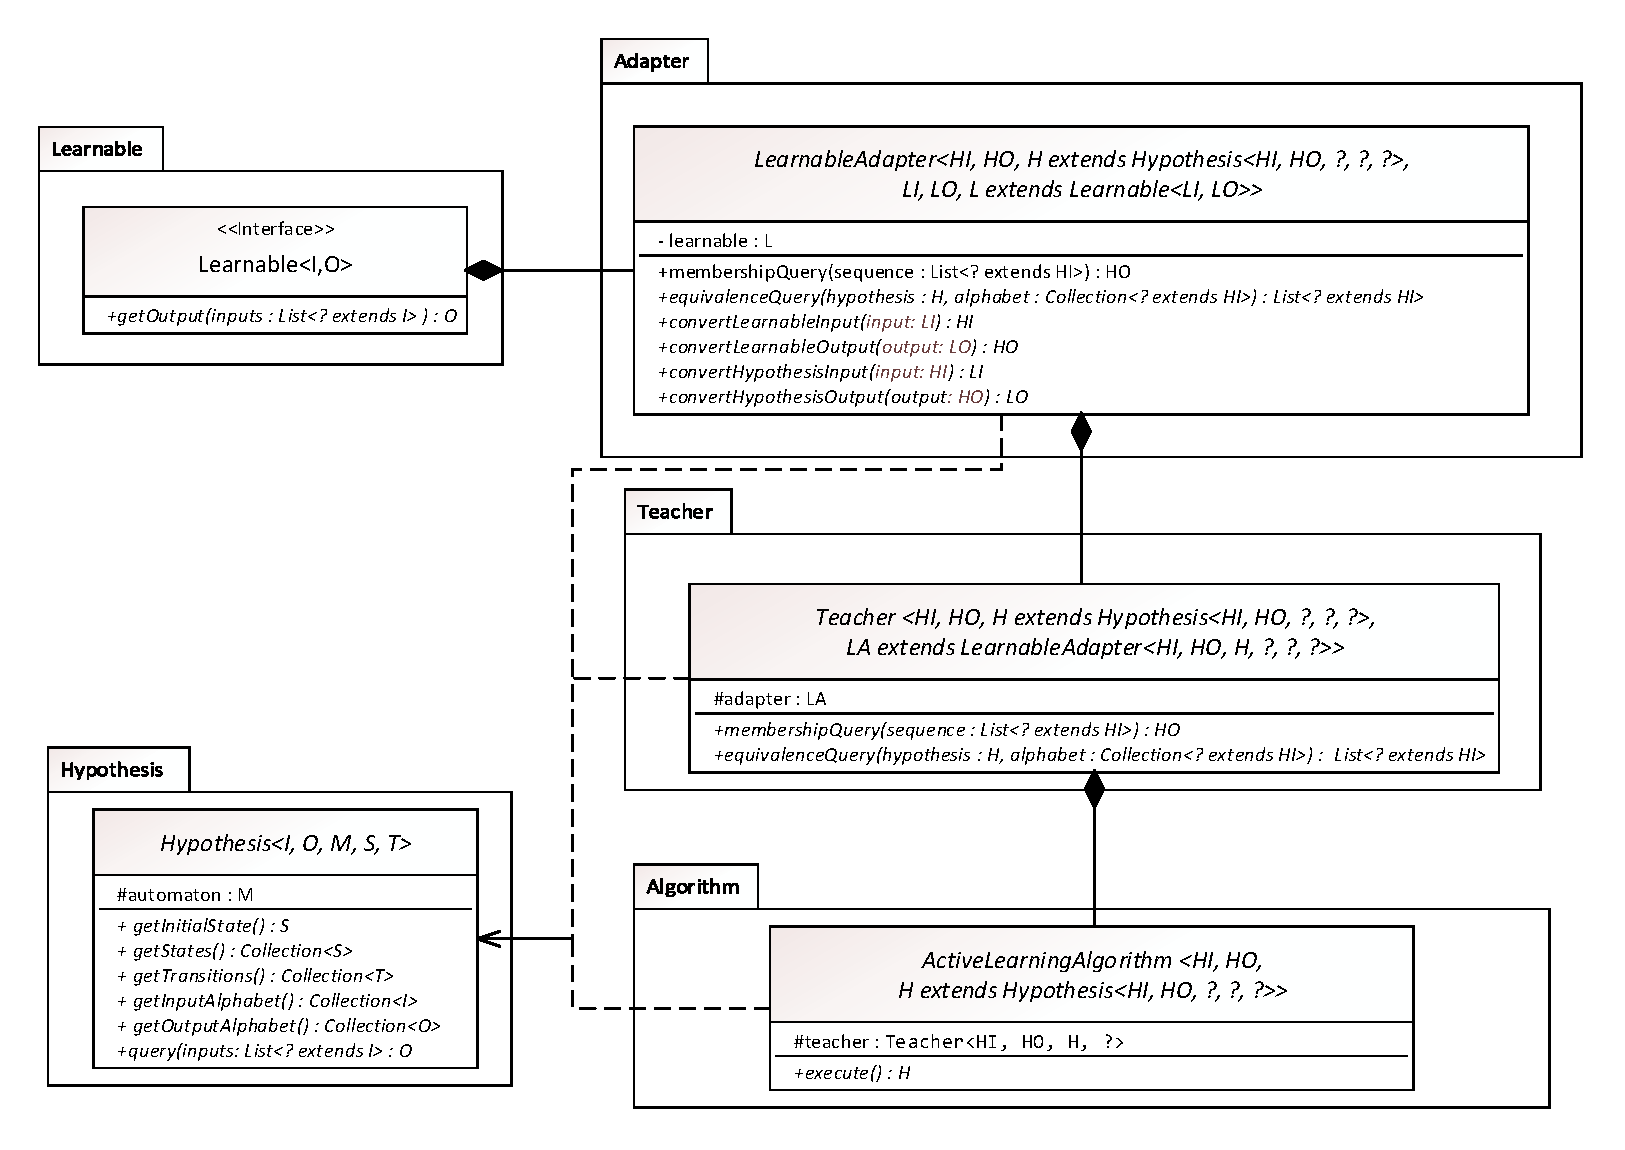
\includegraphics[width=0.97\linewidth]{figures/abstractdetailedoverview}
	\caption{Overview of the abstract classes and interfaces of the framework.}
	\label{fig:abstractdetailedoverview}
\end{figure}

\subsection{Detailed overview of implementation} \label{item:stringsequencelearnable}

The detailed (but not exhaustive) class diagram of the frameworks implementation can be seen in Fig. \ref{fig:abstractdetailedoverview}. The figure is self-explanatory in some regards, while the generic specifics and implementation details are explained in the following.

\begin{itemize}
	\item \textbf{StringSequenceLearnable:} The \emph{StringSequenceLearnable} class is a realization of the Learnable interface, defining simply any type of learnable, which use Strings (java.lang.String) as both input and output types. It contains a simple implementation for describing behavior, accepting a String in the format of $"|input1|output1|input2|output2|...|inputn|outputn|"$, and storing it in a HashMap. One example of this formalism can be seen in Fig. \ref{fig:alternatingbit}.
	
	\item \textbf{MealyLearnable:} The \emph{MealyLearnable} class is a \emph{Learnable} which uses the EMF-modeled \emph{MealyMachine} class seen in Fig. \ref{fig:mealyecore}. Since this implementation of Mealy machines uses Strings as both input and output characters, it extends upon the generic bounds provided by the \emph{StringSequenceLearnable} class.
	
	\item \textbf{DHCHypothesis:} The \emph{DHCHypothesis} abstract class contains the abstractions the DHC algorithm needs to be separated from the implementation of the output formalism. Output here is also implementation-dependent, for DFAs it would be the state after running an input, for Mealy machines it would be output after running an input. Contrary to the \emph{Adapter} layer of input formalisms, every algorithm must define its own abstract hypothesis type, an example being this (the \emph{DHCHypothesis}) class.
	
	\item \textbf{DHCMealyMachineHypothesis:} The \emph{DHCMealyMachineHypothesis} class straightforwardly extends \emph{DHCHypothesis} using the EMF-modeled \emph{MealyMachine} class seen in Fig. \ref{fig:mealyecore}. Essentailly, \emph{DHCMealyMachineHypothesis} is the Mealy machine extension of the DHCHypothesis abstract class, implementing every abstract method of both its superclasses.
	
	\item \textbf{StringSequenceAdapter:} The \emph{StringSequenceAdapter} abstract class adapts \emph{StringSequenceLearnable}s (bounds these using generics), while not defining any generic bounds to the \emph{Hypothesis} it adapts to. This makes it possible to implement equivalance queries only once for every input formalism, using the abstract \emph{convert...()} methods to be implemented by subclasses. The current implementation uses a brute-force method of comparing the outputs of the \emph{Learnable} and the \emph{Hypothesis} for every possible input under the input alphabet. This implementation can be seen in \ref{li:eqbruteforce}.
	
	\item \textbf{StringSequenceToMealyAdapter:} The \emph{StringSequenceToMealyAdapter} class bounds the \emph{Hypothesis} parameters of the \emph{LearnableAdapter} to \emph{DHCMealyMachineHypothesis}, as the dependency relation indicates in Fig. \ref{fig:abstractdetailedoverview}. It only implements the \emph{convert...()} functions.

	\item \textbf{MealyMachineTeacher:} The \emph{MealyMachineTeacher} abstract class bounds the generic parameters of the \emph{Hypothesis} (H) to \emph{DHCMealyMachineHypothesis}, while leaving the \emph{Learnable} (LA) parameter unbound, analogously to \emph{StringSequenceAdapter}. This is done, so algorithm implementations are completely separated from input types. 
	\item \textbf{MealyMachineTeacherStringSequenceImpl:} The \emph{MealyMachineTeacherStringSequenceImpl} class defines the LA generic parameter to be a \emph{StringSequenceAdapter}, and delegates both its methods to it.
	 
	\item \textbf{DirectHypothesisConstruction:} The \emph{DirectHypothesisConstruction} class implements the DHC algorithm using the \emph{DHCHypothesis} abstract class to build its hypothesis. The \emph{constructHypothesis()} method is an implementation of Algorithm \ref{algo:dhc}, constructing a \emph{DHCHypothesis} in a black-box way using the splitters field. The splitters field is initialized and constructed the way described in Algorithm \ref{algo:dhc}, on the first run initialized by the input alphabet, then extended on hypothesis refinement. The \emph{refineHypothesis()} method does exactly this: it takes a counterexample, and adds the suffixes of it to the \emph{splitters}, so the next run of \emph{constructHypothesis()} will split states as needed. The \emph{execute()} method ties everything together by executing \emph{constructHypothesis()}, equivalence queries and the \emph{refineHypothesis()} method. The implementation of the \emph{execute()} method can be seen in Fig. \ref{li:executedhc}.
\end{itemize}

\begin{lstlisting}[caption=The \emph{execute()} function of the DHC algorithm implementation described in Section \ref{item:stringsequencelearnable}s \emph{DirectHypothesisConstruction} item.,label=li:executedhc]
public DHCHypothesis execute() {
	List<? extends I> counterExample = null;
	DHCHypothesis<I, O, M, S, T> h = null;
	do {
		if(counterExample != null) {
			refineHypothesis(counterExample);
		}
		h = constructHypothesis();
		
		counterExample = teacher.equivalenceQuery(h, alphabet);
	}while(counterExample != null);
	
	return h;
}
\end{lstlisting}

\begin{figure}
	\centering
	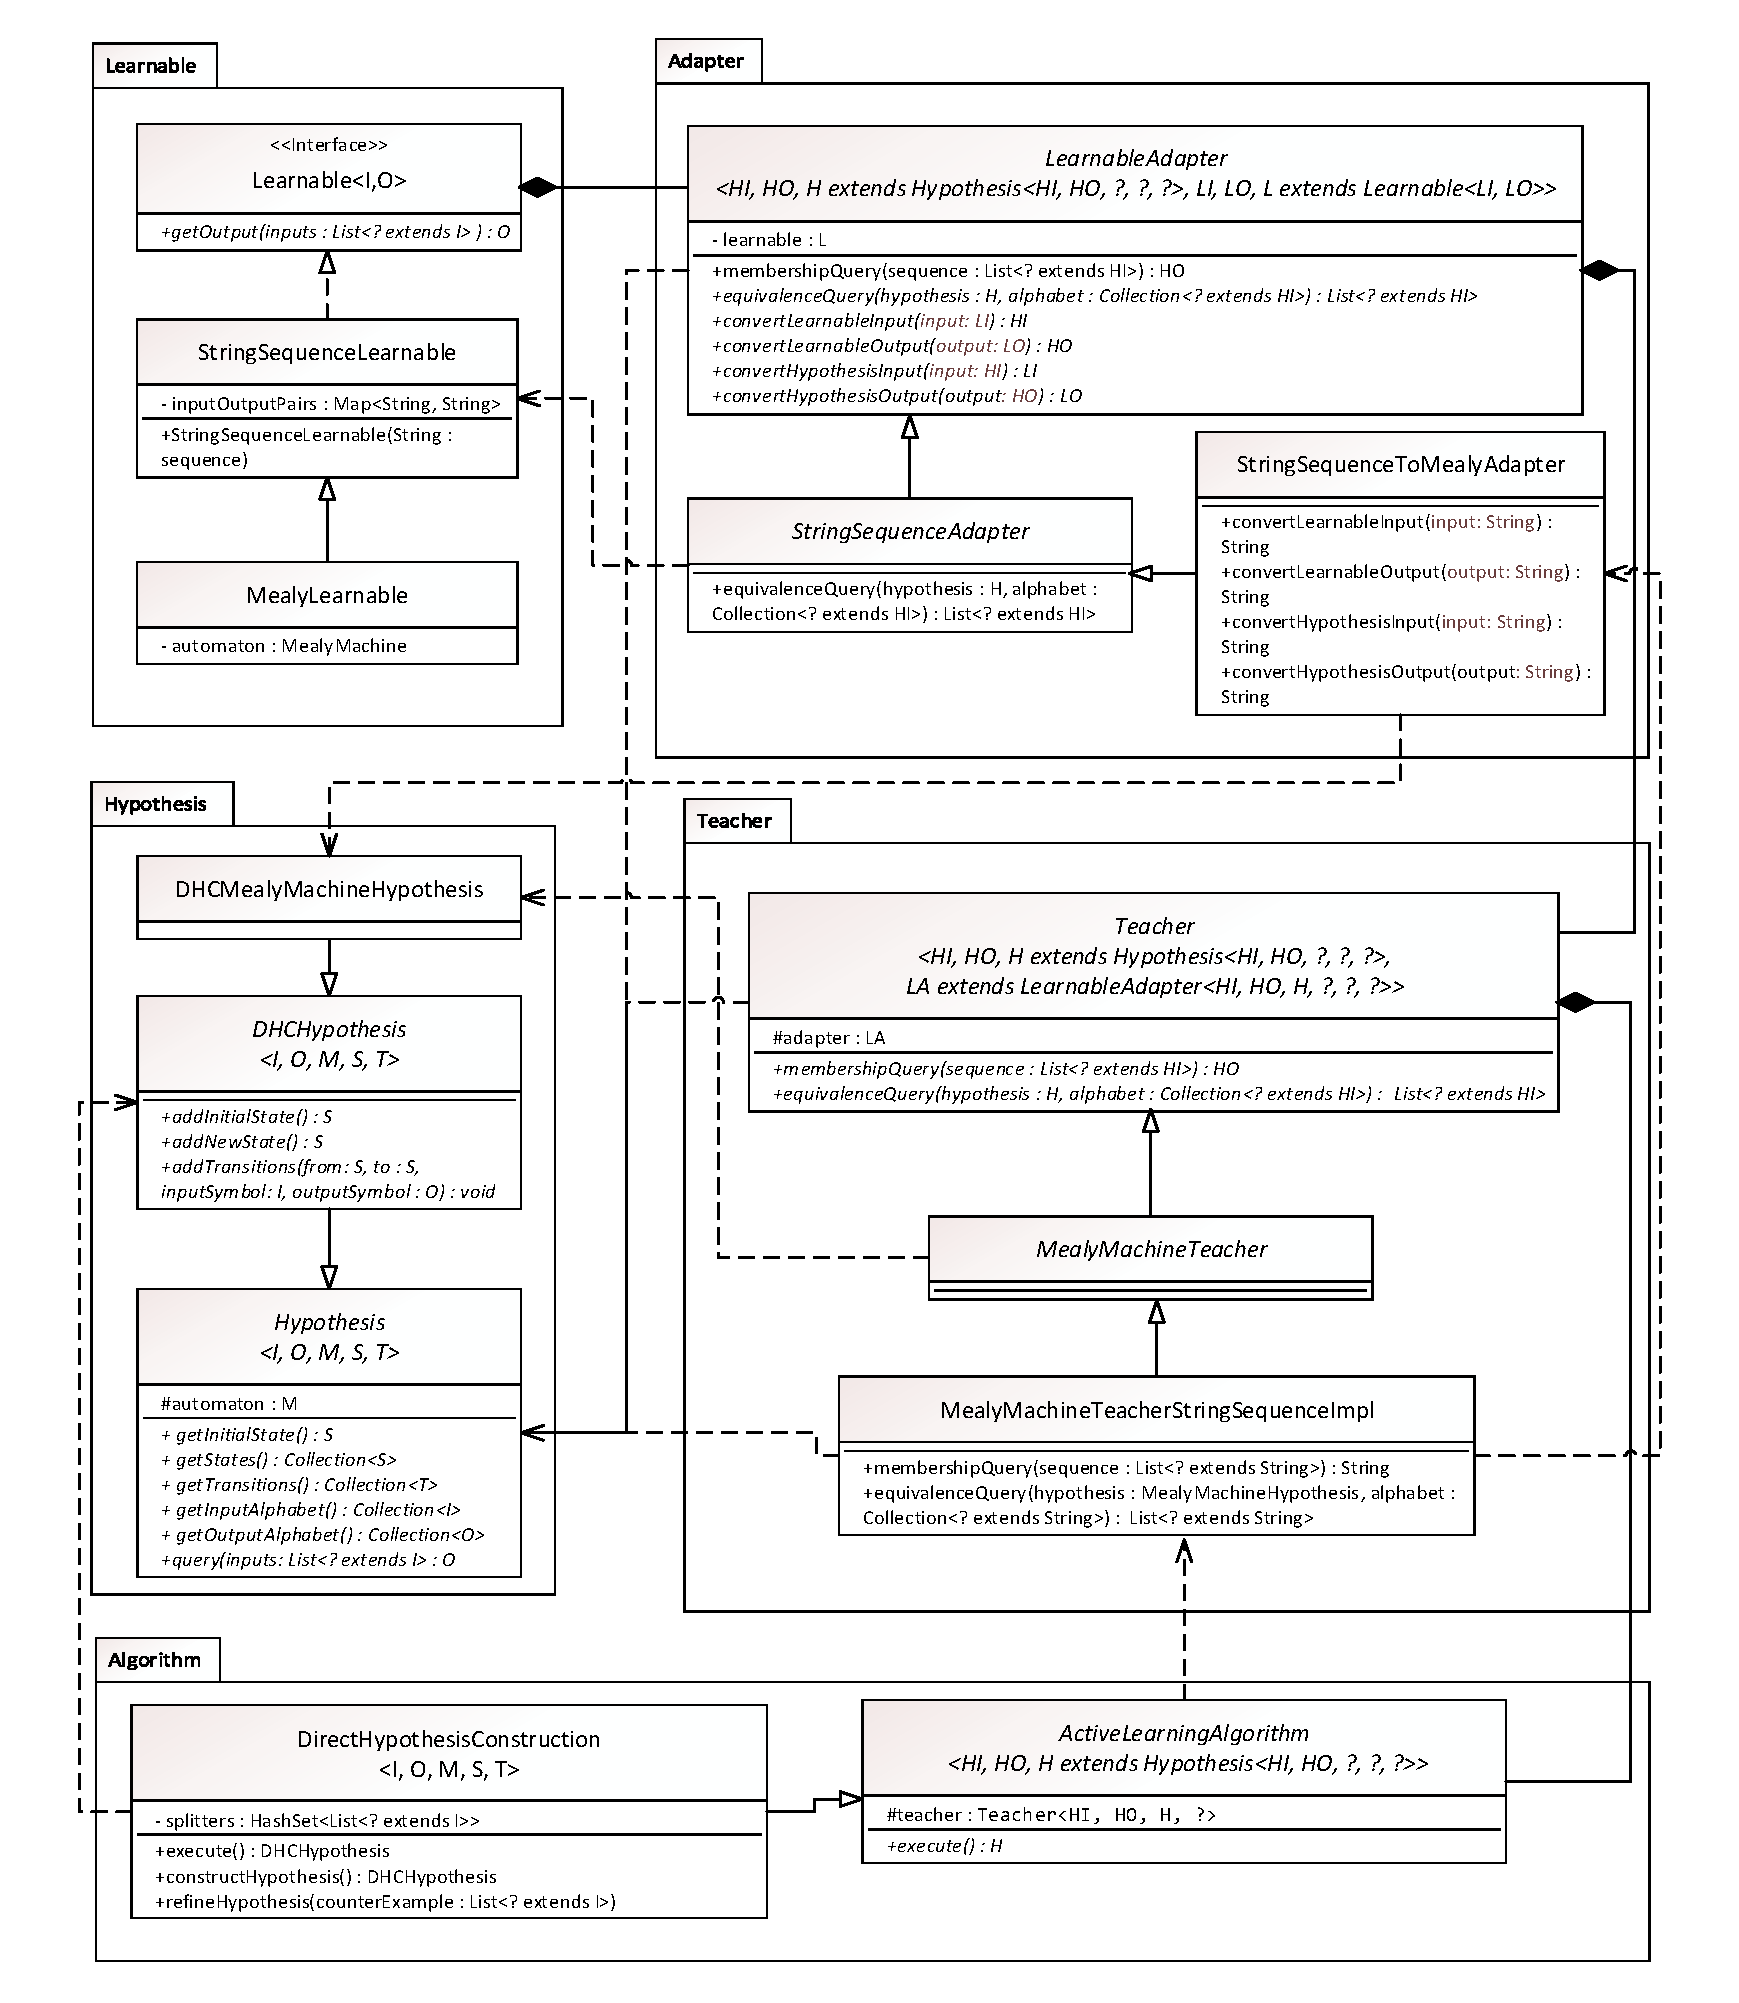
\includegraphics[width=1.0\linewidth]{figures/implementationdetailedoverview}
	\caption{Non-exhaustive detailed overview of the implementation and structure of the framework.}
	\label{fig:impldetailedoverview}
\end{figure}

\chapter{Evaluation}

\section{Theoretical evaluation}

The framework presented in this thesis has both advantages and disadvantages in design and implementation. The modular setup shown in Fig. \ref{fig:abstractoverview}, while providing easy extensibility, does require knowledge of the algorithms implemented therein. In contrary to LearnLib, where (from my experience) data structures are easily extended and onboarded to the learning, algorithm implementations are difficult to provide new solutions to, my framework allows extensibility on every front of it, with a steeper learning curve even with new input/output onboarding.

The framework, when implementing similar formalisms does require some redundancy, especially with the \emph{Learnable-LernableAdapter-Teacher} trio of implementation needed with new formalisms. The advantage of this sometimes redundant approach is the overall elimination of typecasting and uncertain genericity, allowing for exact application of methods and classes after bounding the generic parameters required, improving runtime, the compliance with object-oriented paradigms, and understandibility of an implementation without context of its abstrations. The \emph{Learnable} and \emph{Hypothesis} endpoints of input and output formalisms being interfaces provide flexibility by leveraging the multiple-inheritance (implementation) property of interfaces. This is used for example in the TTT implementation in order to extend upon classes of LearnLib, while still implementing my frameworks abstractions.

\subsection{Evaluation of DHC}

The Direct Hypothesis Construction algorithm, as theorized and proved in \cite{Steffen2011} and \cite{10.1007/978-3-642-34781-8_19}, terminates after at most $n^3mk+n^2k^2$ membership, and $n$ equivalence queries, where $n=|S|$, $k=|\Sigma|$ and m is the longest counterexample. The runtime complexity of these queries are difficult to evaluate, since they highly depend on implementation and context. Reaching the system under learning in the current implementation of input formalisms (String sequece or Mealy machine) takes no overhead, since the system behavior is stored in-memory. This might not be the case in other implementations, where the SUL might be reached through network communication or other such (non-negligible overhead) methods. In terms of membership queries, the current implementations differ. 

String sequences (\emph{StringSequenceLearnable}s) are stored in an input-output \emph{HashMap}, which allows $O(1)$ access assuming the values are evenly distributed in the buckets used by the hashing, worst-case scenario being $O(k)$. While access is fast, this method suffers in terms of space complexity, storing a numer of elements identical to $\mathcal{P}(\Sigma)\setminus\emptyset$, or in text, the powerset of $\Sigma$ without the empty set, resulting in a space complexity of $O(2^k)$.

The MealyMachine implementation (the \emph{MealyLearnable} class) provides a more reasonable $O(k)$ space complexity, but it struggles with runtime issues. The implementation, as discussed in the contribution section, provides ease of access to its data, with straightforward implementation of membership queries possible, not storing the automata in a graph-like format reduces efficiency. This results in a worst-case scenario of an $O(kt)$, where $t$ is the number of transitions of the automaton.

From the perspective of equivalence queries, the two implemented input formalisms both provide the same efficiency, since the implementation of this query is in the \emph{StringSequenceAdapter} class, both \emph{MealyLearnable} and \emph{StringSequenceLearnable} are queried using this implementation, which can be seen in Listing \ref{li:eqbruteforce}. This implementation is a brute-force way of proving equivalence of the hypothesis and the system under learning, operating by taking every permutation of every element in $\mathcal{P}(\Sigma)\setminus\emptyset$ and comparing outputs using membership queries for each of them. In order to mitigate some of this inefficiency, the implementation uses google guavas \emph{Sets.powerSet()} method, providing $O(k)$ space complexity as opposed to a brute-force $O(2^k)$ implementation. For each member of $\mathcal{P}(\Sigma)\setminus\emptyset$, the permutations are calculated using the \emph{Collections2.permutations()} method of guava, implementing the Johnson–Trotter algorithm. This results in a $O(2^kk!)$ number of membership queries considering the "worst case" of finding no counterexamples.

In summary, the best-case scenario of the current DHC implementation has an $O(n^3mk^2+n^2k^3+2^kk!k)$ runtime complexity, the worst case being $O(n^3mk^2t+n^2k^3t+2^kk!kt)$ depending on the variables presented above.

\subsection{Evaluation of TTT}

The TTT algorithm, as presented in \cite{10.1007/978-3-319-11164-3_26}, requires $O(n)$ equivalence queries and $O(kn^2+n\log m)$ membership queries, each of which takes $O(n+m)$ time, where $n=|S|$, $k=|\Sigma|$ and m is the longest counterexample. This is a very pessimistic estimate caused by the edge-case of a discriminator tree having $n$ height. The time complexity of the equivalence query implementation seen in \ref{li:eqbruteforce} still holds as $O(2^kk!)$, but is lengthened by the complexity of conversion between formalisms, being $O(nt)$ in the worst case, where t is the number of transitions of the current hypothesized automaton. Altogether, the worst case scenario has a $O((kn^2+n\log m)(n+m) + 2^kk!nt)$ time complexity. TTT also provides an efficient $\Theta(kn)$ space complexity\cite{10.1007/978-3-319-11164-3_26}.

\chapter{Conclusions}
This chapter concludes the contributions of this thesis, and presents myfuture goals.

\section{Contributions}
%saját kontribúció pontokban szedve
%tudományos kontribúció pontokban sedve
%2mondat. As a result, lehetővé tettem, van egy keretrendszer...
\section{Future work}
%további algoritmusok, gamma intergráció közelebbről távolabbra. (keretrendszertől absztrakthozt)

% Acknowledgements
%~~~~~~~~~~~~~~~~~~~~~~~~~~~~~~~~~~~~~~~~~~~~~~~~~~~~~~~~~~~~~~~~~~~~~~~~~~~~~~~~~~~~~~
%%----------------------------------------------------------------------------
\chapter*{\koszonetnyilvanitas}\addcontentsline{toc}{chapter}{\koszonetnyilvanitas}
%----------------------------------------------------------------------------

Ez nem kötelező, akár törölhető is. Ha a szerző szükségét érzi, itt lehet köszönetet nyilvánítani azoknak, akik hozzájárultak munkájukkal ahhoz, hogy a hallgató a szakdolgozatban vagy diplomamunkában leírt feladatokat sikeresen elvégezze. A konzulensnek való köszönetnyilvánítás sem kötelező, a konzulensnek hivatalosan is dolga, hogy a hallgatót konzultálja.


% List of Figures, Tables
%~~~~~~~~~~~~~~~~~~~~~~~~~~~~~~~~~~~~~~~~~~~~~~~~~~~~~~~~~~~~~~~~~~~~~~~~~~~~~~~~~~~~~~
%\listoffigures\addcontentsline{toc}{chapter}{\listfigurename}
%\listoftables\addcontentsline{toc}{chapter}{\listtablename}


% Bibliography
%~~~~~~~~~~~~~~~~~~~~~~~~~~~~~~~~~~~~~~~~~~~~~~~~~~~~~~~~~~~~~~~~~~~~~~~~~~~~~~~~~~~~~~
\addcontentsline{toc}{chapter}{\bibname}
\bibliography{bib/mybib}


% Appendix
%~~~~~~~~~~~~~~~~~~~~~~~~~~~~~~~~~~~~~~~~~~~~~~~~~~~~~~~~~~~~~~~~~~~~~~~~~~~~~~~~~~~~~~
%----------------------------------------------------------------------------
\appendix
%----------------------------------------------------------------------------
\chapter*{\fuggelek}\addcontentsline{toc}{chapter}{\fuggelek}
\setcounter{chapter}{\appendixnumber}
%\setcounter{equation}{0} % a fofejezet-szamlalo az angol ABC 6. betuje (F) lesz

%\numberwithin{tabular}{section}

\begin{lstlisting}[caption=The Mealy machine seen in Fig.\ref{fig:coffeemealy} in the form of the Xtext the grammar described in Listing \ref{li:xtext}.,label=li:coffeemealy]
MealyMachine{
initialState 
State a states { State a, State b, State c, State d, State e, State dd, State f
}inputAlphabet Alphabet { characters { water , pod , button , clean } }
outputAlphabet Alphabet { characters { done , coffee , none } }
transitions{ 
Transition { input clean output done sourceState a targetState a } , 
Transition { input pod output done sourceState a targetState b } , 
Transition { input water output done sourceState a targetState c } , 
Transition { input button output none sourceState a targetState f } , 
Transition { input pod output done sourceState b targetState b } , 
Transition { input water output done sourceState b targetState d } , 
Transition { input button output none sourceState b targetState f } , 
Transition { input clean output done sourceState b targetState a } , 
Transition { input clean output done sourceState c targetState a } , 
Transition { input pod output done sourceState c targetState dd } , 
Transition { input button output none sourceState c targetState f } , 
Transition { input water output done sourceState c targetState c } , 
Transition { input water output done sourceState d targetState d } , 
Transition { input pod output done sourceState d targetState d } , 
Transition { input clean output done sourceState d targetState a } , 
Transition { input button output coffee sourceState d targetState e } , 
Transition { input water output done sourceState dd targetState dd } , 
Transition { input pod output done sourceState dd targetState dd } , 
Transition { input button output coffee sourceState dd targetState e } , 
Transition { input clean output done sourceState dd targetState a } , 
Transition { input clean output done sourceState e targetState a } , 
Transition { input button output none sourceState e targetState f } , 
Transition { input pod output none sourceState e targetState f } , 
Transition { input water output none sourceState e targetState f } , 
Transition { input clean output none sourceState f targetState f } , 
Transition { input button output none sourceState f targetState f } , 
Transition { input pod output none sourceState f targetState f } , 
Transition { input water output none sourceState f targetState f } } }
\end{lstlisting}



%\label{page:last}
\end{document}
